\begin{frame}{Data Split}
\begin{itemize}
    \item To ensure your model doesn’t overfit to the training data, you should have another subset called \textbf{testing data}.
    \item You will evaluate your model against this \textbf{subset}, and based on its \textbf{metric score (e.g., accuracy)} you will decide if it’s overfitting or not.
    \item But how should I split my data?
\end{itemize}
\end{frame}


\begin{frame}{Data Split}
\begin{itemize}
    \item \textbf{Hold-out set:}
    \begin{itemize}
        \item A portion of the dataset set aside and not used during training.
        \item E.g. 80\% for training and 20\% for testing.
    \end{itemize}

    \item \textbf{Issues:}
    \begin{itemize}
        \item Imagine you have these labels: [1, 1, 2, 2, 2, 3, 3, 3, 3, 3] and you took last 30\% as test: [3,3,3]. \textcolor{red}{You didn’t include 1 and 2 in test}!
        \item \textbf{Solution:} Always shuffle before split: [3, 2, 3, 1, 3, 2, 3, 1, 3, 2] $\Rightarrow$ test: [1,3,2]
        \item \underline{My dataset is small}. Taking 20\% as test would not be representative!
        \item \textbf{Solution:} Use \texttt{KFold}.
    \end{itemize}
\end{itemize}
\end{frame}

\begin{frame}{Data Split}
\begin{itemize}
    \item \textbf{K-Fold Cross Validation (CV):}
    \begin{itemize}
        \item Split data into $k$ parts (folds)
        \item Train on $k - 1$ folds, test on the remaining fold
        \item Repeat $k$ times and average the scores
    \end{itemize}
\end{itemize}

\begin{figure}
    \centering
    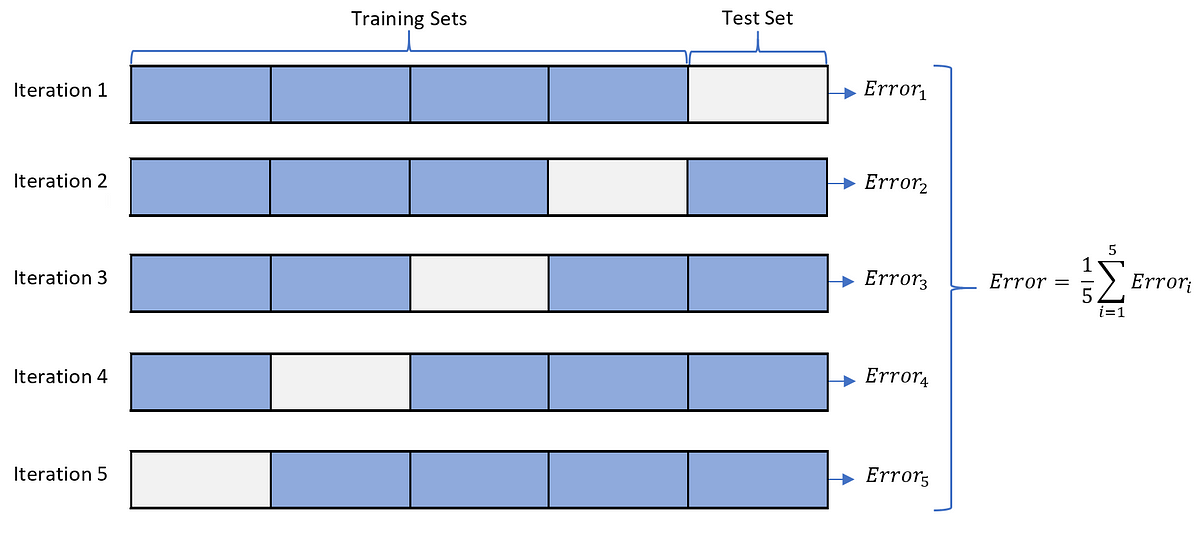
\includegraphics[width=0.9\linewidth]{images/linear-regression/linear-regression-21.png}
\end{figure}
\end{frame}
